%++++++++++++++++++++++++++++++++++++++++s\\
\documentclass[letterpaper,12pt]{article}
\usepackage{tabularx} % extra features for tabular environment
\usepackage{amsmath}  % improve math presentation
\usepackage{graphicx} % takes care of graphic including machinery
\usepackage[margin=1in,letterpaper]{geometry} % decreases margins
\usepackage{cite} % takes care of citations
\usepackage[final]{hyperref} % adds hyper links inside the generated pdf file
\usepackage{caption}
\usepackage{float}
\usepackage{subcaption}
\usepackage{hyperref}
\hypersetup{
	colorlinks=true,       % false: boxed links; true: colored links
	linkcolor=blue,        % color of internal links
	citecolor=blue,        % color of links to bibliography
	filecolor=magenta,     % color of file links
	urlcolor=blue         
}
%++++++++++++++++++++++++++++++++++++++++


\begin{document}

\title{732A75 Advanced Data Mining laboratory 3 report}
\author{Yuki Washio (timwa902) and Nicolas Taba (nicta839)}
\date{\today}
\maketitle



\section{Introduction}

The aim of this laboratory exercise is to test the limits of the clustering algorithm using the distance metric and understand that the clustering algorithms can sometimes fail to provide clusters that correspond to classes that we (humans) may intuit better.

In order to illustrate this, we are using the MONK dataset. The dataset is presented on \href{https://archive.ics.uci.edu/ml/datasets/MONK's+Problems}{the UCI machine learning repository} as well as more in-depth for our particular problem in \href{https://www.researchgate.net/publication/2293492_The_MONK's_Problems_A_Performance_Comparison_of_Different_Learning_Algorithms}{this article}.
This dataset presents 124 data points associated to 7 categorical attributes for the purposes of classification. The MONK1 dataset is used to try to classify (class 0 or class 1) using the following constraints: a1 = a2 and a5 = 1, where a1, a2, a5 are attributes of the data points.

We will first start an exploratory analysis and clustering using appropriate clustering methods for our problem using the distance as a metric and trying to improve on it as much as possible before turning to assosciation analysis.


\section{Clustering}

The dataset presents categorical data. We should use hierarchical clustering methods to create our clusters and obtain the desired 2 clusters.

We are going to use the complete link and kmeans that use euclidean distance as a metric for 2 clusters.

\begin{figure}[H]
\begin{subfigure}{.5\textwidth}
  \centering
  % include first image
  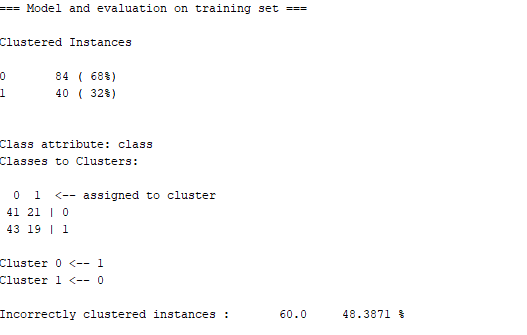
\includegraphics[width=.8\linewidth]{hierarch_complete_link_results}  
  \caption{complete link hierarchical clustering}
  \label{fig:sub-first_1}
\end{subfigure}
\begin{subfigure}{.5\textwidth}
  \centering
  % include second image
  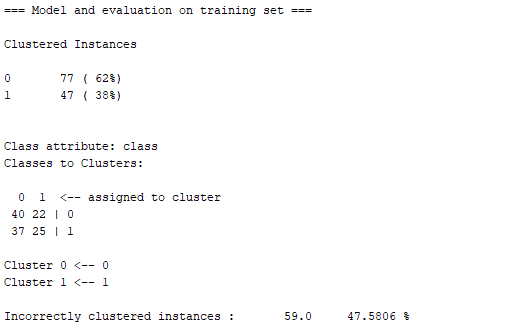
\includegraphics[width=.8\linewidth]{hierarch_kmeans_results}  
  \caption{kmeans clustering}
  \label{fig:sub-second_1}
\end{subfigure}
\caption{Results of clustering algorithm}
\label{fig:fig_1}
\end{figure}

The clustering algorithm does not perform well and guesses incorrectly about half of the time. This is very bad performance because it is only slightly better than a random guess. This is because although some of the attributes of some data points are similar, they belong to different classes. We cannot distinguish the different class instances using distance as a metric in this case.

We can slightly improve the clustering by creating an outlier cluster. We also use single link hierarchical clustering. This improves the performance of the clustering algorithm, but is still not sufficient enough.



\begin{figure}[H] 
  \centering
      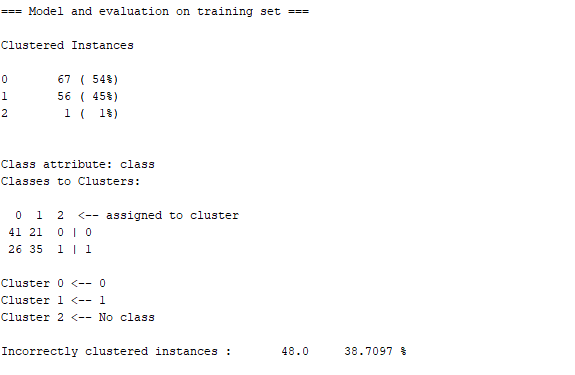
\includegraphics[width=0.8\columnwidth]{hierarch_single_link_3clusters_results}
        \caption{
                \label{fig:best_single_link}  
                Single link hierarchical clustering
        }
\end{figure}

The performance improves from random guess to 62\% accuracy.

\section{Assosciation analysis}

We perform association analysis using the apriori algorithm and find up to 19 rules using a minimum support of 0.05. The rules created are presented in Fig.\ref{fig:assosciation_rules}.

\begin{figure}[H] 
  \centering
      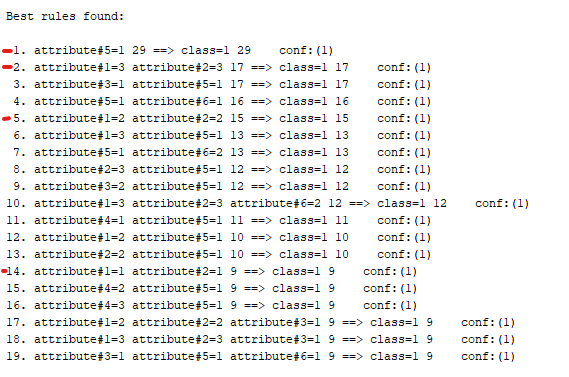
\includegraphics[width=0.8\columnwidth]{apriori_lab3}
        \caption{
                \label{fig:assosciation_rules}  
                19 best assosciation rules for MONK1 dataset.
        }
\end{figure}

Since this is a binary problem, it is sufficient to study rules that predict class 1. We were able to find 4 rules that describe class 1 (the support of these rules covers all the cases of class 1). The rules that describe class 1 are marked in red in Fig.\ref{fig:assosciation_rules} and are the same than the expected rules in the description of the dataset in \url{https://www.researchgate.net/publication/2293492_The_MONK's_Problems_A_Performance_Comparison_of_Different_Learning_Algorithms}
.


\section{Discussion}

The clustering algorithm has failed to predict when considering the problem of predicting the class. The algorithm might however give us more insights into other aspects of the dataset. The clustering algorithm fails because some of the attributes are not necessary to the classification. Using distance is not a proper measure to establish class differences.

Association analysis and the establishment of rules gives us in this case a more robust way of classifying the data.


\end{document}
